\chapter{Linear Acceleration}

\section{Aim}
To learn how to determine the linear acceleration of a body

\section{Background Information}
A body is said to undergo acceleration if its velocity changes. Any change of motion is associated with a force. When the force on a moving object remains constant with time its velocity increases constantly. What happens to its acceleration? 

\section{Materials}
Ticker timer with paper tape, flat smooth board, pencil, trolley, pulley, scale pan, 500 g mass, string 

\section{Procedure}
\begin{enumerate}
\item Fix a 50 Hz ticker timer and a trolley onto a 2 m long smooth horizontal board.
\item Tie a strip of paper tape from the ticker timer to one end of the trolley and a piece of string to the other end of the trolley as shown in Figure \ref{fig:linear-acceleration-1}. 
\item Attach a pulley to the end of the horizontal board. Place the string over the pulley.
\item Attach a scale pan onto the loose end of the string. While holding the pan in your hand, place a 500 g mass into the pan. Do not let go of the pan.
\item Switch on the vibrator of the ticker timer.
\item Let go of the pan so that it falls to the floor. 
\item Observe the dots made on the tape by the ticker timer and label every 10 consecutive dots on the tape using a pencil (Ignore the first few dots, see Figure \ref{fig:linear-acceleration-2})
\item Measure the distances between the points AB, BC and CD occupied by successive 10 dot-spaces.
\end{enumerate}

\begin{figure}[h!]
\centering
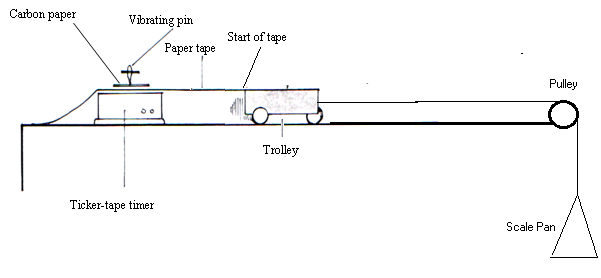
\includegraphics[width=14cm]{./img/linear-acceleration-1.png}
\caption{Linear Acceleration practical setup}
\label{fig:linear-acceleration-1}
\end{figure}

\begin{figure}[h!]
\centering
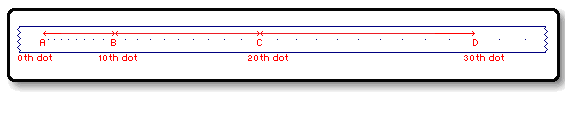
\includegraphics[width=14cm]{./img/linear-acceleration-2.png}
\caption{Example ticker timer tape}
Note: The dots are 0.02 seconds apart.
\label{fig:linear-acceleration-2}
\end{figure}

\section{Analysis and Interpretation}
\begin{enumerate}
\item Find the distance between points A and B and calculate the average velocity during that time interval. Label it $V_1$. 
\item Repeat step 1 above for BC and CD and calculate the velocities in each section. Label them accordingly. 
\item Find the rate of change of velocity between each section. Comment on the values.
\item Calculate the average acceleration at points B, C and D by using the total change in distance multiplied by 2 and divided by the total time squared. (i.e. $a=2\times \Delta s\slash \Delta t^2$).
\item Find the difference between the distances traveled between AB and BC. Divide by the period squared. Comment on the value. 
\item Repeat step 5, but this time between the distances traveled between BC and CD.
\item Comment on the values obtained in steps 3, 4 and 5.
\end{enumerate}

\section{Conclusion}
From this experiment what is the acceleration of the trolley?

\section{Questions for Discussion}
\begin{enumerate}
\item What causes the trolley to accelerate?
\item Under what condition is the acceleration of the trolley zero?
\item Do you expect there to be a relationship between the mass in the pan and the acceleration of the trolley? Explain your answer.
\item How does friction affect the results of this experiment?
\end{enumerate}

\section{Reflection and Self Assessment}
\begin{enumerate}
\item Is there anything you do not understand in this experiment? If so, what is it and what can you do to increase your understanding?
\item What were the most and least interesting parts of this experiment to you? Explain.

\end{enumerate}